\documentclass{tpu-sotu}
\usepackage{ascmac}
\usepackage{cite}
\usepackage[dvipdfmx]{hyperref}
\usepackage[dvipdfmx]{graphicx}
\usepackage{pxjahyper}
\usepackage{siunitx}
\usepackage{listings}%begin{lstlisting}で使える
\lstset{
language=C,%
basicstyle={\small},% 
identifierstyle={\small},% 
commentstyle={\small\ttfamily \color[rgb]{0,0,0}},% 
keywordstyle={\small\bfseries \color[rgb]{0,0,1}},% 
ndkeywordstyle={\small},% 
stringstyle={\small\ttfamily}, 
frame={tb}, 
breaklines=true,
columns=[l]{fullflexible},% 
numbers=left,%これ消すと行番号消える
xrightmargin=0zw,% 
xleftmargin=3zw,% 
numberstyle={\scriptsize},% 
stepnumber=1, 
numbersep=1zw,% 
morecomment=[l]{//}% 
}

\title{UPPAALを用いた自動運転車の\\群制御アルゴリズムのモデル化と検証}
\etitle{Modeling and verification \\of autonomous-vehicle group control algorithms using UPPAAL}
\author{佐原 優衣}
\gakusekibangou{1515024}
\date{平成31年(2019年)2月}
\professor{中村 正樹 准教授}
\department{電子・情報工学科}
%- - - - - - - - - - - - - - - - - - - - - - - - -

\begin{document}
\maketitle
\clearpage

\pagenumbering{roman}
\setcounter{tocdepth}{3}
\tableofcontents
\clearpage
\pagenumbering{arabic}

\chapter{はじめに}
	\section{背景}
	自動運転技術は発達し続けている。自動運転は,搭載される技術によってレベル1からレベル5までに分けられており,現在,日本国内では,運転者支援を主としたレベル2までが市販車に採用されている。今後,高速道路や,限定地域での特定条件下での完全自動運転を行うレベル4の車両の普及が目指されている。
	
	完全自動運転の普及の環境の一例として,アラブ首長国連邦において再生可能エネルギーを利用し,二酸化炭素を排出しないゼロカーボンを目指すマスダールシティプロジェクトが2006年に始まった。マスダールはアラブ首長国連邦の一つアブダビ首長国の首都アブダビの近郊で図\ref{Masdar}の様な人口約5万人,面積約6.5\si{km^{2}}の人工都市として計画されている。
	
	このプロジェクトでは道路交通は自動運転車のみで構成される予定である。住民が任意の時刻に自動運転車に乗降し都市空間内を移動することを想定しているため,大量の車両の配備が必要となる。道路上の車両密度が高くなるため,渋滞やデッドロックが発生することが想定される。したがって,個々の車両だけではなく,自動運転車群が効率的に走行するアルゴリズムが必要となる。
	
	しかし,効率的に制御された自動運転車が安全かどうかアルゴリズムから一目では判断しきれない。そこで本研究では群制御アルゴリズムが欲しい性質を持っているかどうかを検証する手法を提案する。
	\begin{figure}[htbp]
	\centering
	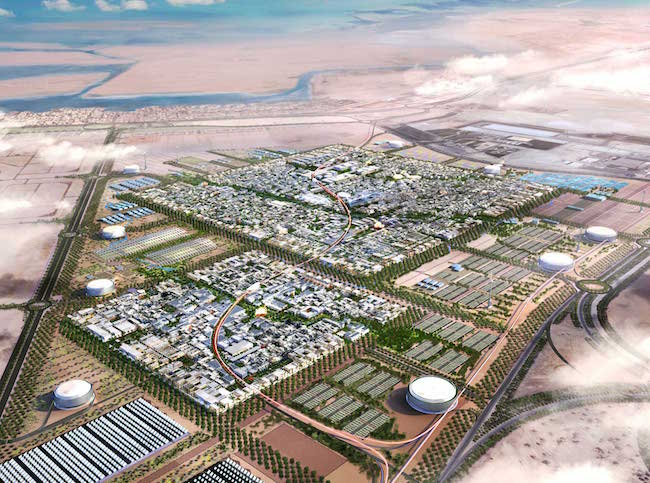
\includegraphics[width=130mm]{Masdar.jpg}
	\caption{マスダール・シティの完成イメージ \protect \footnotemark}
	\label{Masdar}
	\end{figure}
	\footnotetext{出典:Masdar社}
	\section{目的}
	自動運転車の群制御アルゴリズムを形式的に記述し,モデル検査を用いて,性質を検証する。
	\begin{figure}[htbp]
	\centering
	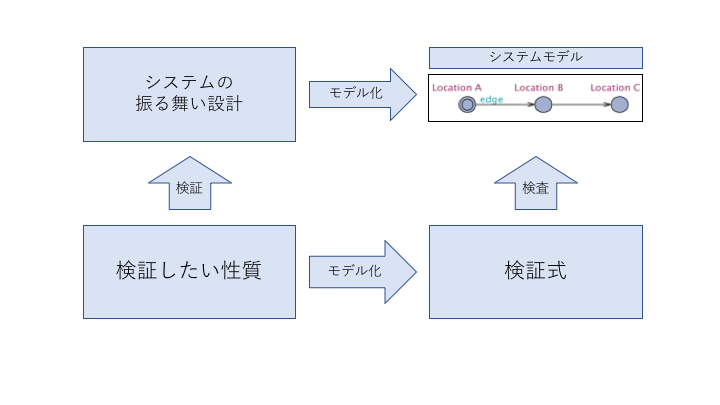
\includegraphics[width=150mm]{ModelVerification.png}
	\caption{モデル検査による形式的な検証}
	\label{ModelV}
	\end{figure}
	\section{論文の構成}
	本論文は,2章で本研究で用いるモデル検査の概説と使用するモデル検査ツールの概説,3章で単一の交差点における車両のモデル化と検証,4章で検証にかかる時間や検証の質,5章でまとめを述べるといった構成である。
\chapter{モデル検査}
本章では文献\cite{a1}からモデル検査とUPPAAL\cite{u1}の概説を行う。
	\section{モデル検査}
	モデル検査は,システム上で起こり得る状態を網羅的に調べることにより設計の誤りを発見する自動検証手法の一種である。モデル検査手法は,システムの振る舞いの設計,および検証したい性質をそれぞれモデル化し,ツールを用いて,システムが性質を満たしているかを調べる。
	
	モデル検査において,システムの動作を表現するシステムモデルを作成する必要がある。ソフトウェア開発のどの段階でモデル検査を活用したいか,もしくは,何をどの程度検証したいかによって,どのような情報をもとにどのようにシステムモデルを作成するかが変わってくる。専用のシステムモデルを入力とするモデル検査を設計モデル検査,ソースプログラムを入力とするモデル検査をプログラムモデル検査と呼ぶ。これらのモデル検査がソフトウェア開発の流れの中での活用例を図\ref{develP}に示す。図\ref{develP}にソフトウェアの品質向上のために行われる手順も挙げた。設計モデル検査は設計レビューを,プログラムモデル検査はコードレビューをそれぞれ補完する位置付けである。
	\begin{figure}[htbp]
	\centering
	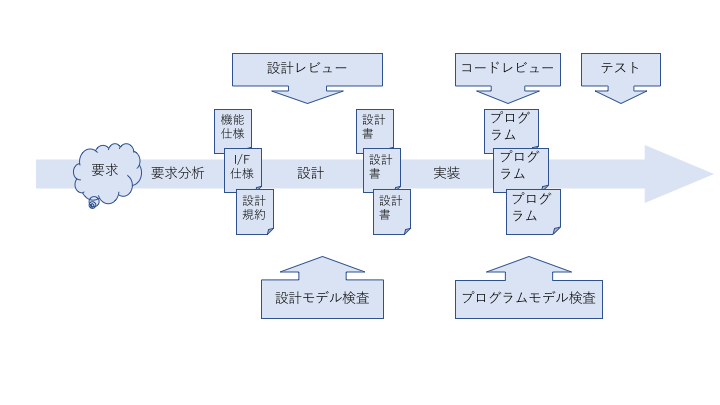
\includegraphics[width=155mm]{developmentProcess.png}
	\caption{ソフトウェア開発プロセス}
	\label{develP}
	\end{figure}
	\subsection{様々なモデル検査ツール}
	次に,いくつかのモデル検査ツールを特徴と共に例示する。代表的なモデル検査ツールには,処理が高速で大規模なモデルを扱えるNuSMV\cite{Nu},並列処理やマルチスレッドの設計モデルを扱えるSPIN\cite{s1},GUIベースの入力による時間制約を扱えるUPPAAL\cite{u2}などがある。
	
	NuSMVは状態遷移図からのモデル化に向いており,また,各状態が満たす論理式などを用いて記号的に検査を行う,莫大な状態数を持つ系に対して検査が可能なシンボリックモデル検査ツールである(図\ref{NuSMV})。
		
	%{SPINはPromelaという専用の言語を用いて検証対象をモデル化する。動作主体を複数定義し,各動作主体の動作はC言語に似た文法で記述される。複数の動作主体の状態の組み合わせの数は,例え一動作主体あたりの状態数が比較的少なくとも,非常に大きくなることが起こりがちである。これを状態爆発と称される。SPINは状態爆発を緩和するために,半順序簡約,ビットステートハッシュ,状態ベクトル圧縮,データフロー・制御フロー解析によるスライシングなどの諸技術が用いられている。}
	\begin{figure}[htbp]
	\centering
	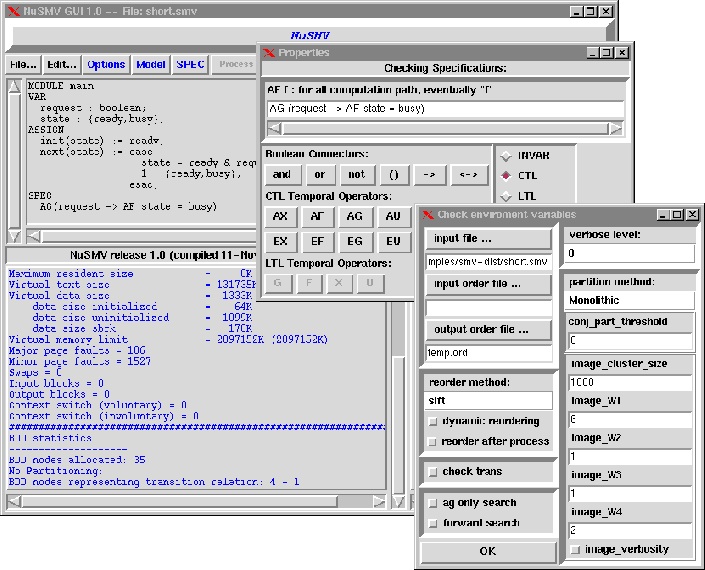
\includegraphics[width=100mm]{NuSMV.png}
	\caption{NuSMVのツール画面\cite{n2}}
	\label{NuSMV}
	\end{figure}
	
	SPINはPromelaという専用の言語を用いて検査対象をモデル化する。SPINの最大の特徴はモデル検査そのものを実施せず,対象を固有のC言語ソースを生成する。メモリ使用量を削減し,性能向上と共に,モデルに使用者が自由にC言語コードを追加できる利点がある(図\ref{SPIN})。
		
	\begin{figure}[htbp]
	\centering
	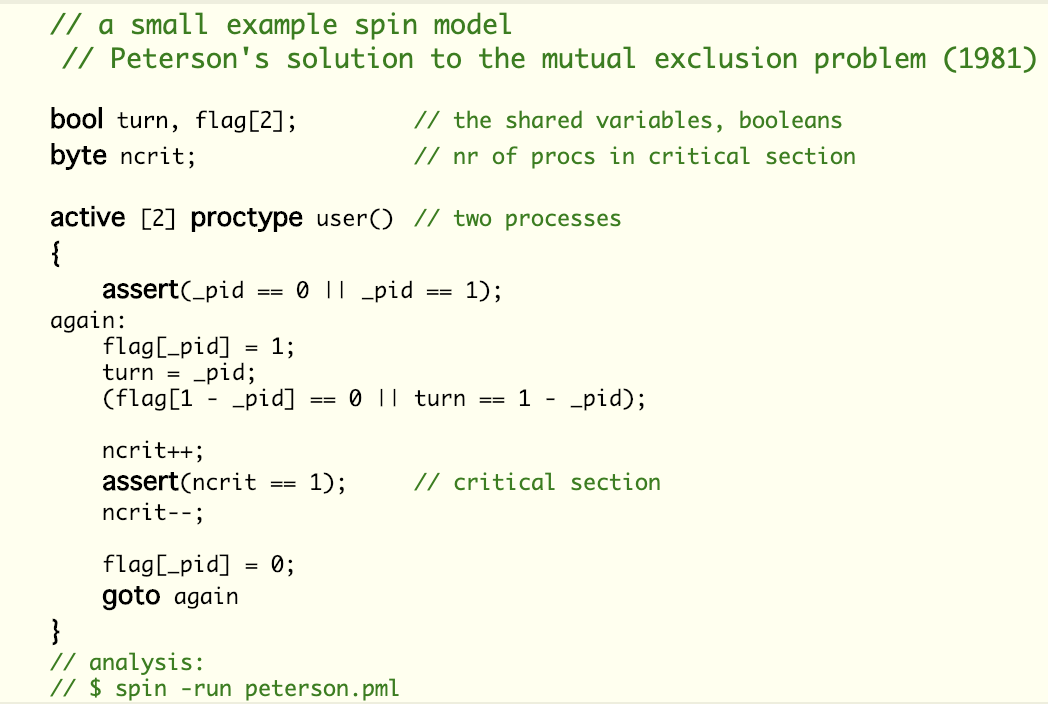
\includegraphics[width=100mm]{SPIN.png}
	\caption{SPINのソースコード\cite{s2}}
	\label{SPIN}
	\end{figure}
	
	UPPAALの最大の特徴である時間が扱えることの利点を記述する。イベントの発生時刻や処理時間,これらの時間的なズレの三点について任意に設定できるため,時間が扱えないモデル検査と違い,応答時間などの時間制約を検証対象にすることが可能である。また,イベントの発生と特定の処理の開始を簡単に記述できる。具体例として,ビジネスプロセスの時間と資源に関する性質のモデル化と検証の適用例などがある\cite{a9}。
	\section{モデル検査ツールUPPAAL}
	本節は,UPPAALについて概説する。UPPAALはシステムモデルの入力をGUIベースにより定義している。このため,作成したシステムモデルが直感的に把握しやすい。入力したシステムモデルに対して,GUIベースでシミュレーション実行とステップ実行が可能である。シミュレーション画面では,各プロセスの現在状態と変数の値,状態遷移図とメッセージシーケンスが表示される。
	
	検証は検証したい性質を検証式で入力する。検証はすべての可能性のある実行パスに対して網羅的に検査を行う。検証結果は,入力した検証式に対して成否が緑か赤で示される。性質に反した場合は,反するまでの実行履歴が反例として示される。反例の表示はシミュレーション画面で行われ,ステップ単位でトレースすることで,各プロセスの状態や変数値の変化を確認可能である。
	また時間制約を含む検証に関して,「最短時間で違反状態に到達する反例の出力」という機能を持つ。通常出力されるのは任意の一種類ではあるが,特に初期状態から検証したい性質に反するまでの経過時間が最短となる反例を出力する機能である。検証したい性質として,「仕事が完了することがない」という条件を与えることにより,仕事が完了する手順が反例となるが,仕事が完了する手順の中で最短時間のものを出力することになる。
	\subsection{UPPAALの操作}
	本節では,例題を用いてUPPAALを使用する。
	
	4台の車が出発地点から到着地点まで,それぞれ違う方向から一つの交差点に進入し,通過するとき4台の車が全て通過し終わるのにかかる最小時間を検証する。なお,この交差点には右折レーン,信号がないものとする。北から南に向かう車ns,南から北にぬける車sn,東から西にぬけるew,西から東にぬけるwe,の4台は時速約30kmほどで走っており,南北同士,東西同士の場合はお互いに止まることなく通過するが,nsとewのような交差する場合は先に交差点への進入権を獲得した方が先に通過することとなる。そのため交差点への進入権をいつ獲得し,交差点の通過にかかる時間も考慮する。
	
	UPPAALはシステムモデルをGUI言語で作成する。UPPAALでは本例題における,車一台一台をエージェントと呼び,一台の車のおける出発地点から目的地まで通過するという一連の動作のことをプロセスと呼ぶ。同一の挙動を示すプロセスの定義を個別に行わなくてもすむように,テンプレートという概念を用いている。そのため,システムモデルの作成では,まずプロセスの挙動を定義したテンプレートの定義から行う。図\ref{CC}では現在選択しているものが青で囲われている。現在はエディタで,テンプレートが選択されている状態である。テンプレートの名前はエディタタブのすぐ下で定義できる。本例題ではCarCouseとする。名前の隣にパラメータが入力部分がある。パラメータは参照渡しを行うことができる。同じテンプレートCarCouseのインスタンスとなる複数のプロセスで,プロセスごとにアクセスしたい変数が違う時に使う。
	\begin{figure}[htbp]
	\centering
	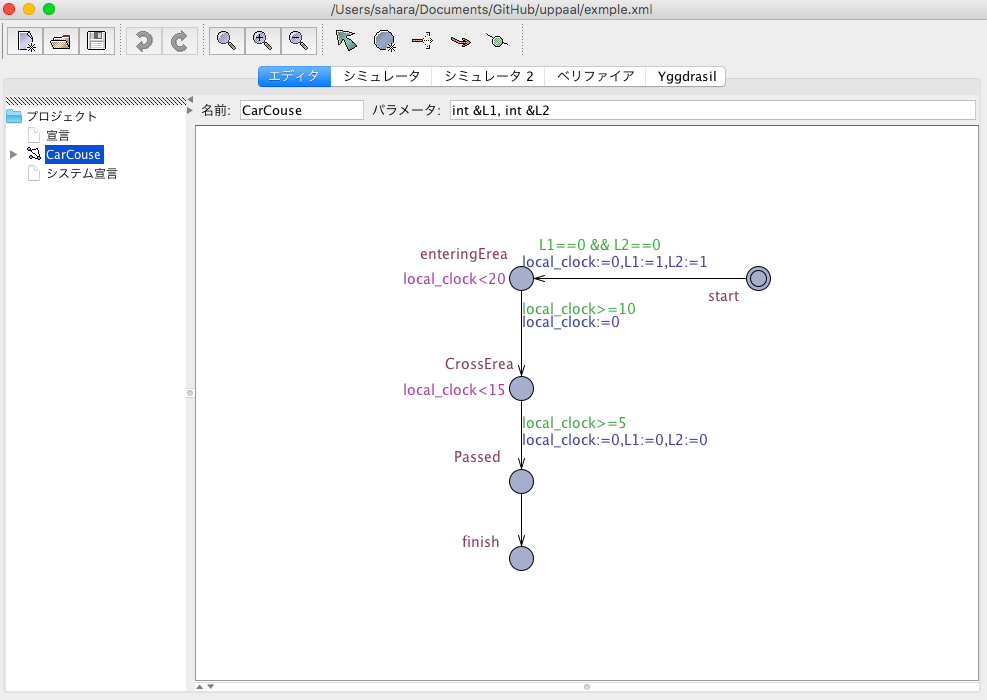
\includegraphics[width=160mm]{CarCouse.png}
	\caption{システムモデルの入力部分}
	\label{CC}
	\end{figure}
	\begin{figure}[htbp]
	\centering
	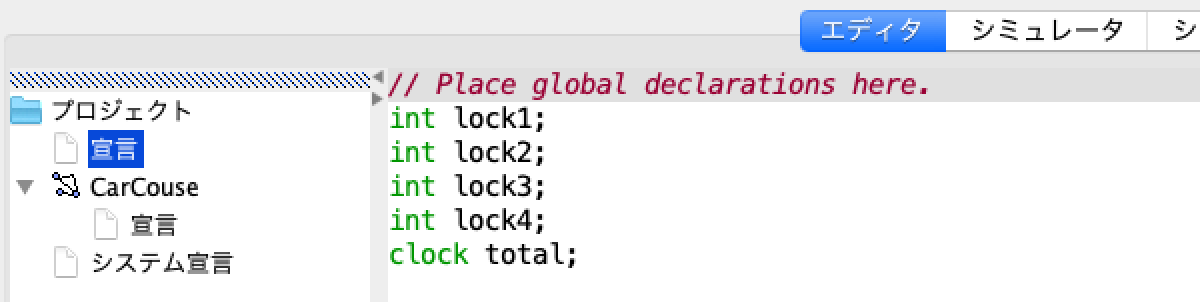
\includegraphics[width=140mm]{GlobalDec.png}
	\caption{大域情報編集ペイン}
	\label{GD}
	\end{figure}
	\begin{figure}[htbp]
	\centering
	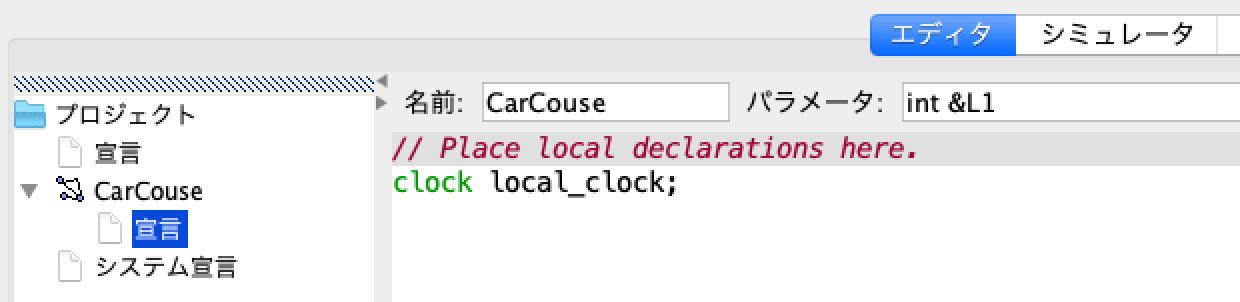
\includegraphics[width=140mm]{LocalDec.png}
	\caption{局所的情報編集ペイン}
	\label{LD}
	\end{figure}
	\begin{figure}[htbp]
	\centering
	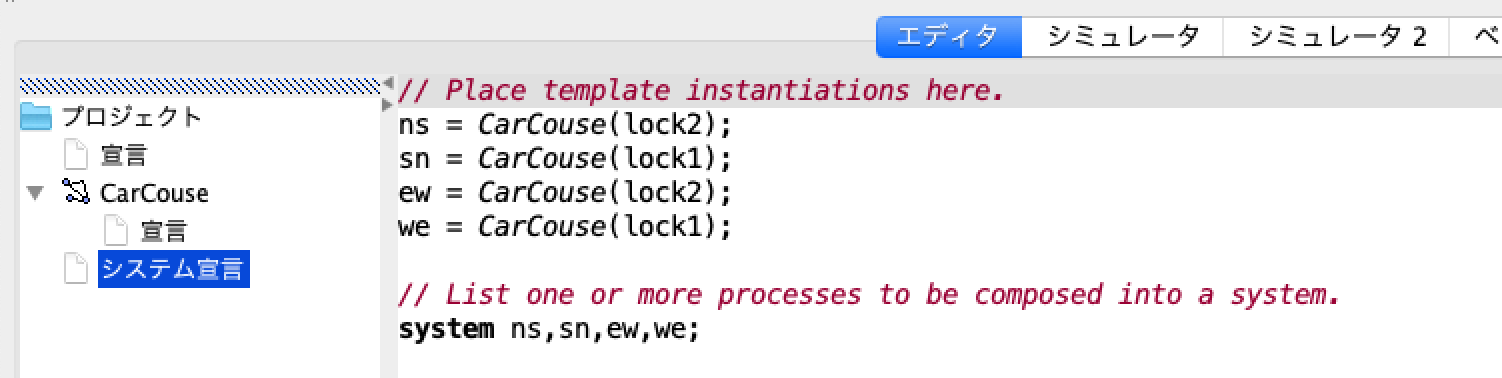
\includegraphics[width=140mm]{SystemDec.png}
	\caption{システム定義編集ペイン}
	\label{SysD}
	\end{figure}
	\begin{figure}[htbp]
	\centering
	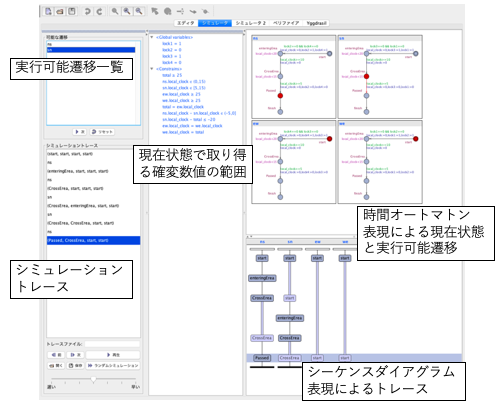
\includegraphics[width=160mm]{ExmpleSimulationResult.png}
	\caption{シミュレーション機能}
	\label{ESR}
	\end{figure}
	\begin{figure}[htbp]
	\centering
	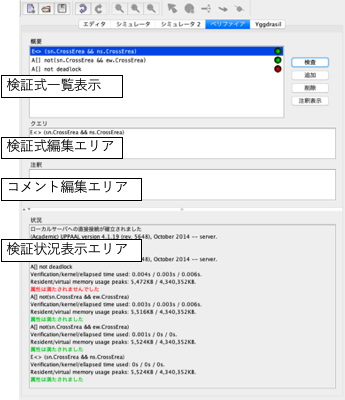
\includegraphics[width=140mm]{showModelVerification.png}
	\caption{モデル検査機能}
	\label{sMV}
	\end{figure}
	シミュレーションと検証:
	
	時間表現:
	
\chapter{群制御アルゴリズムのモデル化と検証}
UPPAALを用いて交差点を通過する1台の自動運転車の挙動をモデル化する。車両
	\section{時間制約のない進行方向を固定しない交差点}
	\begin{figure}[htbp]
	\centering
	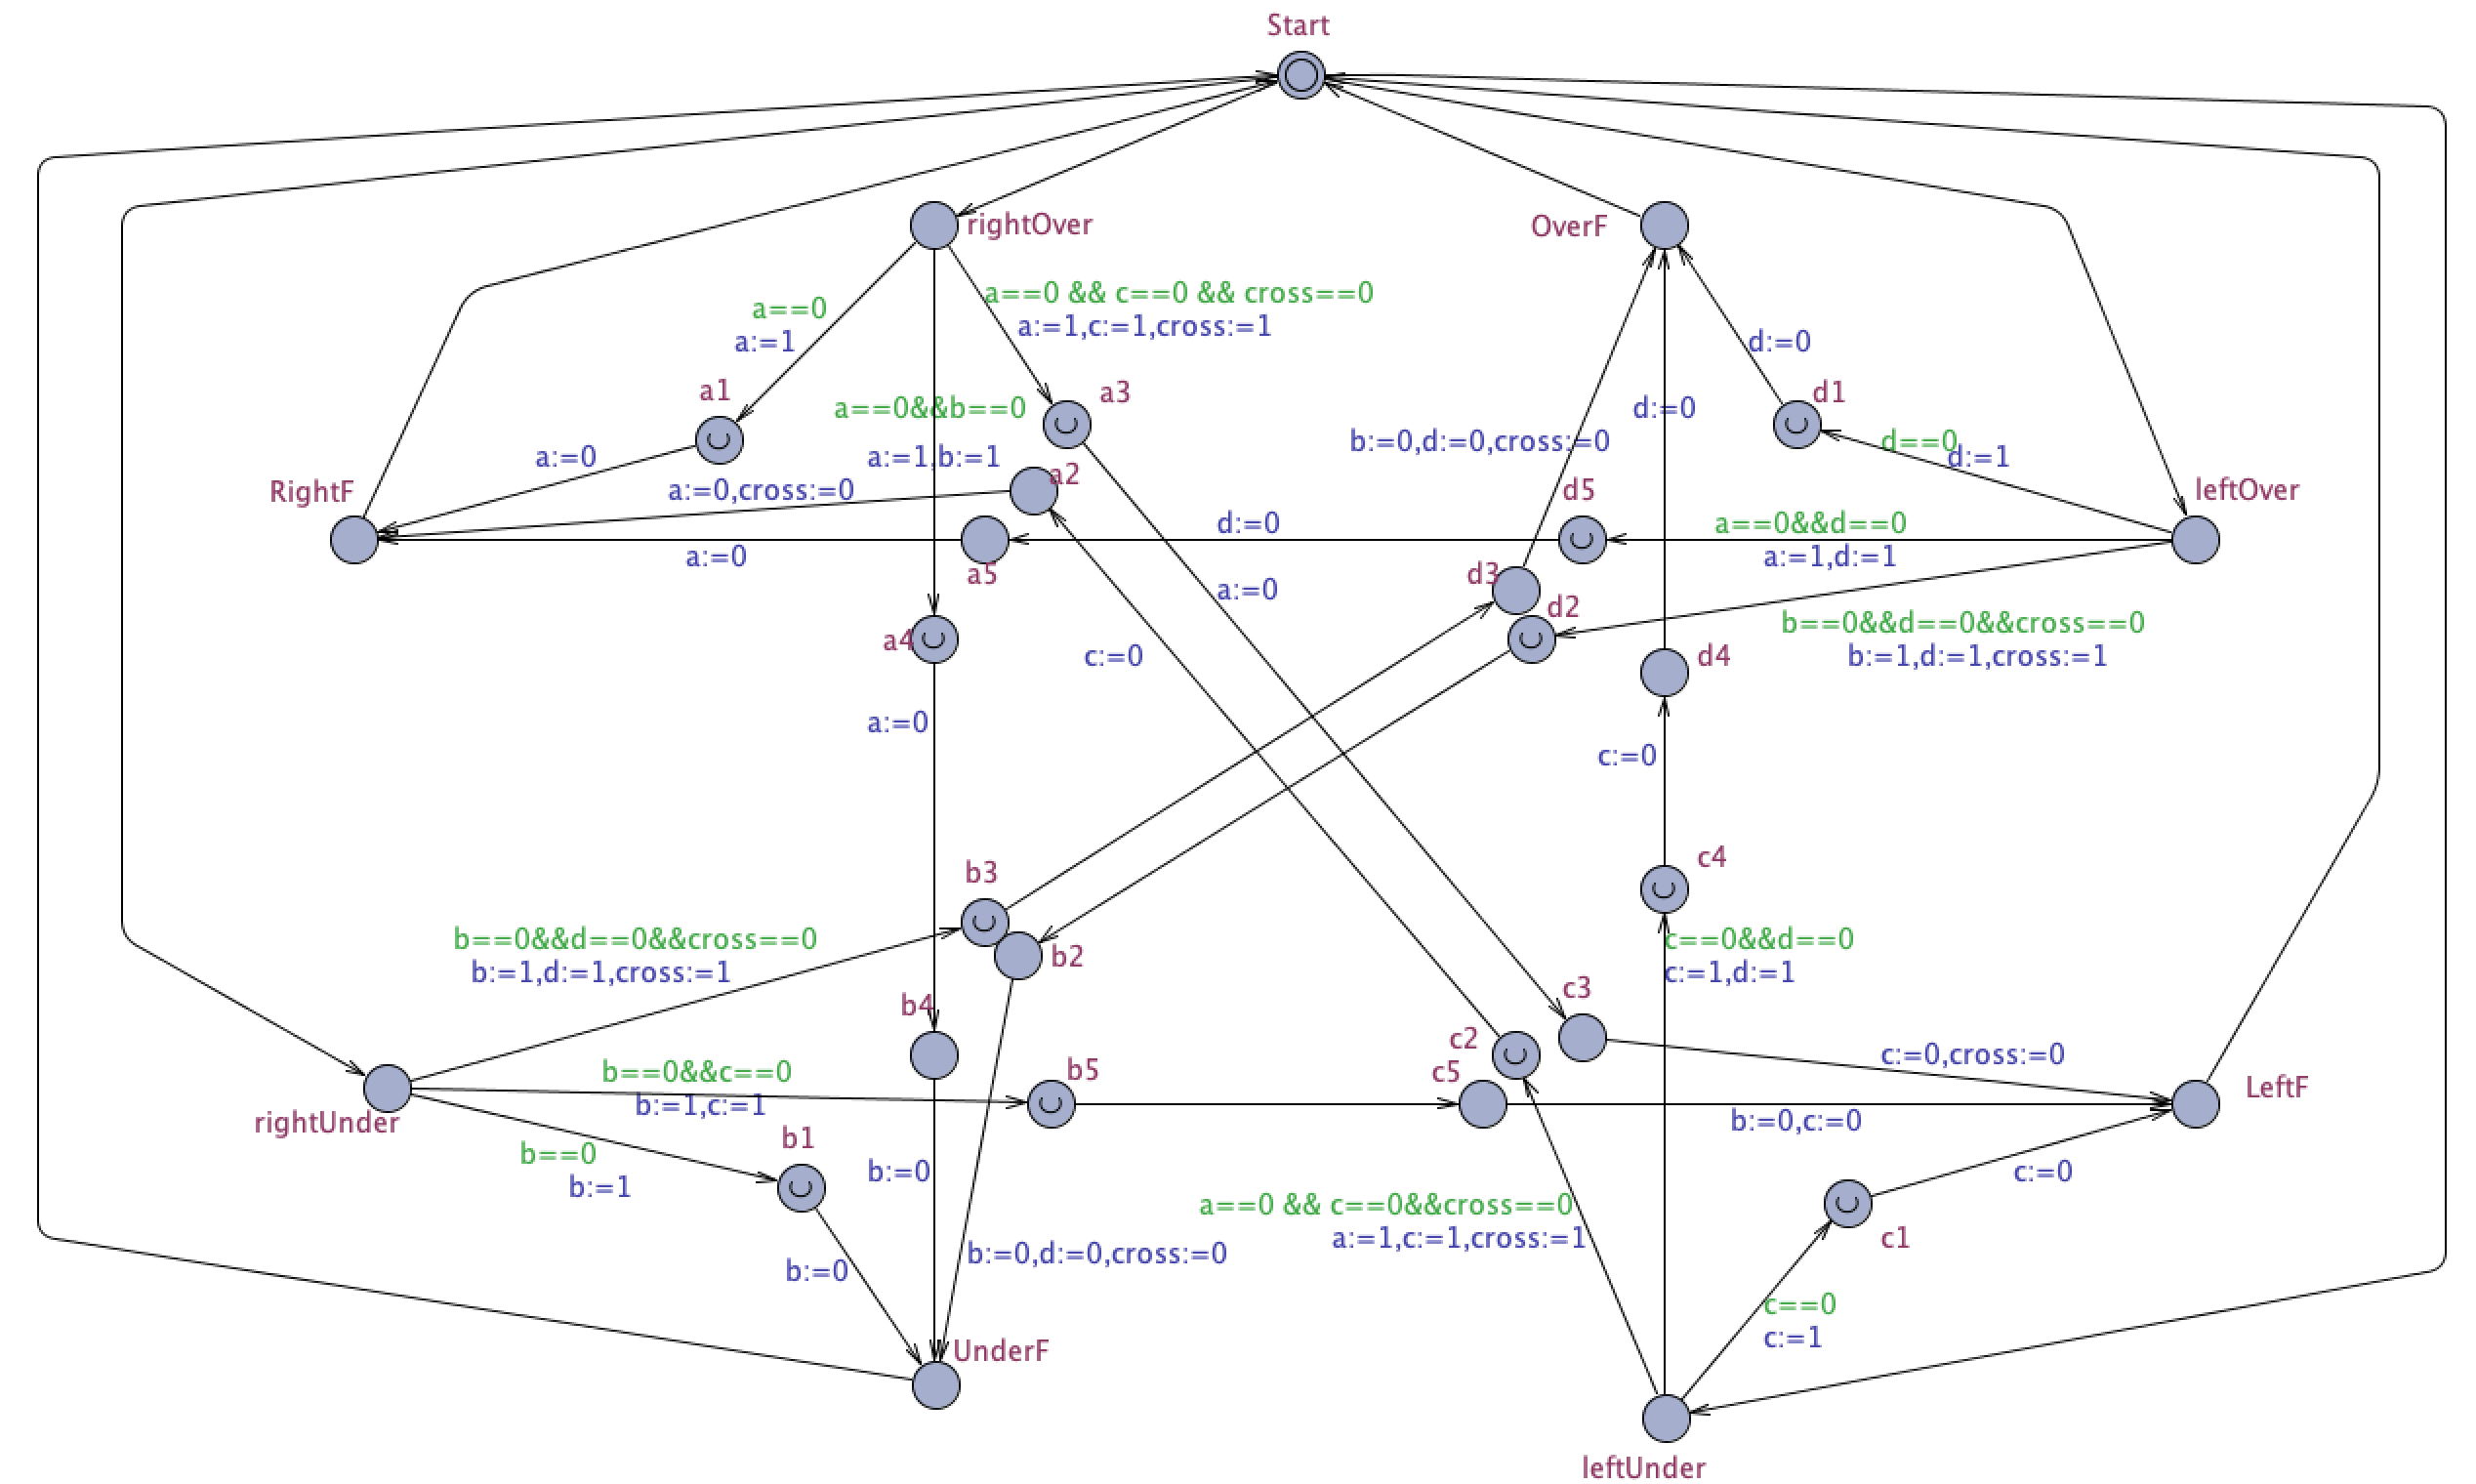
\includegraphics[width=155mm]{IntersectionBig.png}
	\caption{進行方向を固定しない交差点のモデル}
	\label{IB}
	\end{figure}
	
	\begin{figure}[htbp]
	\centering
	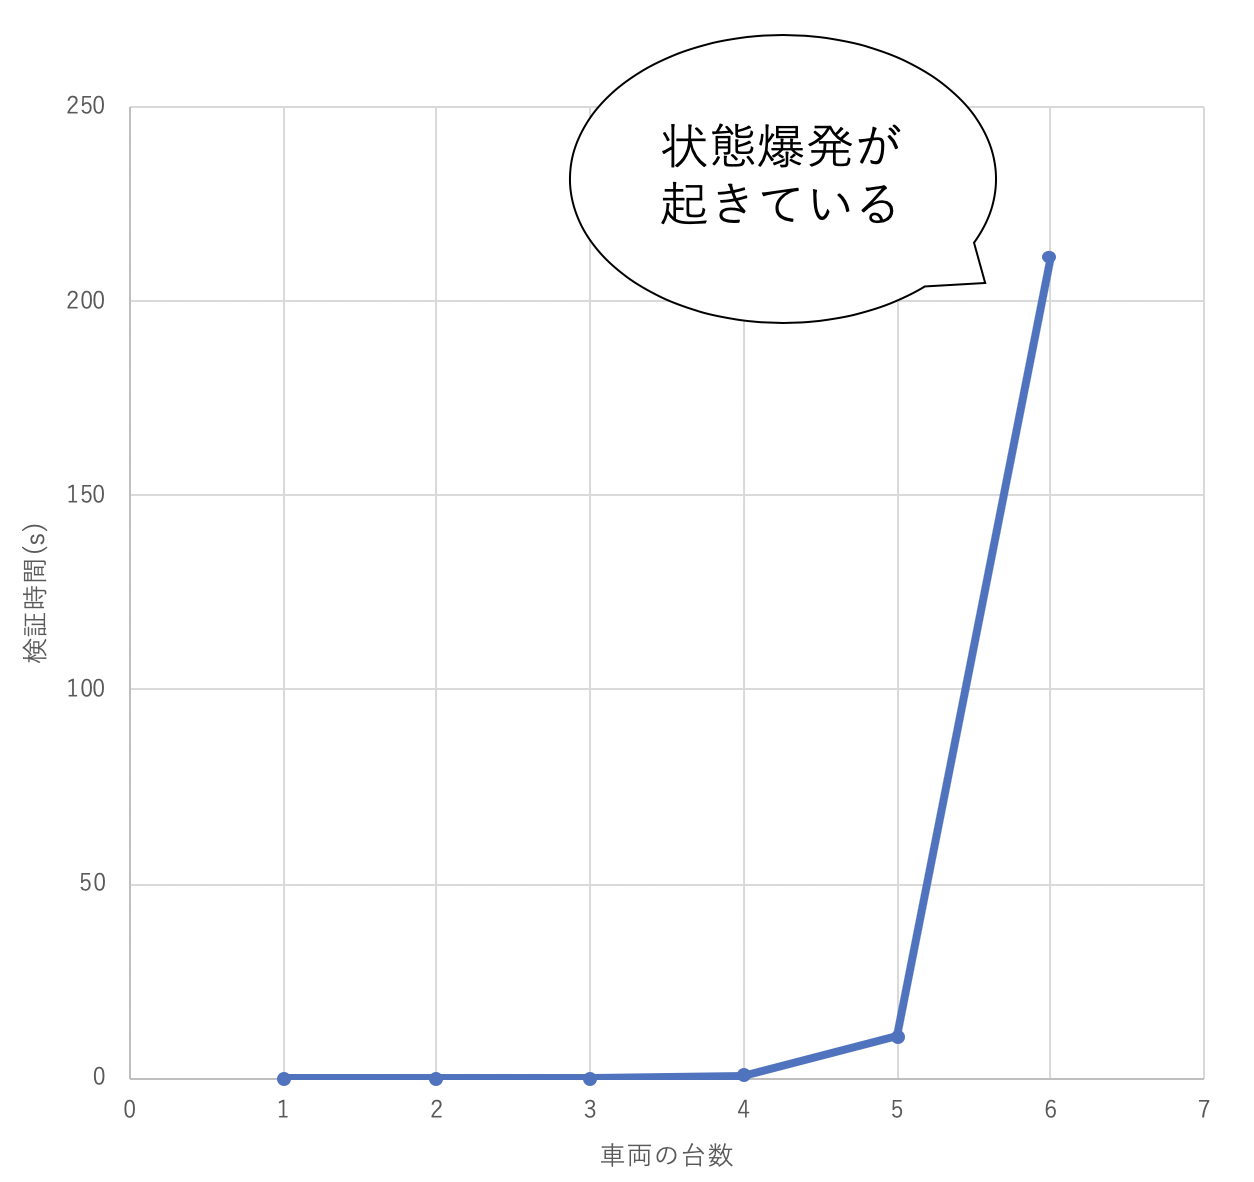
\includegraphics[width=120mm]{IntersectionVerificationTime.png}
	\caption{車両の台数と検証にかかる時間の関係}
	\label{IVT}
	\end{figure}

	\begin{figure}[htbp]
	\centering
	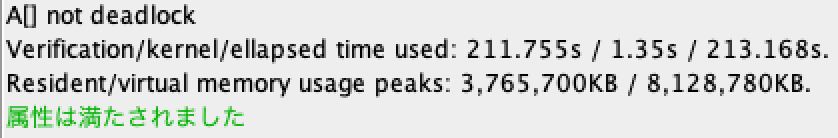
\includegraphics[width=110mm]{InterBigCar6.png}
	\caption{進行方向を固定しない交差点のモデルにおける6台の車両の検証結果}
	\label{IBC6}
	\end{figure}

	
	\section{時間制約を用いる進行方向を固定する交差点}
	本節では,交差点に進入する車両の進行方向を固定して,時間オートマトン\cite{u3}を作成する。車両1台の挙動は,交差点進入前,交差点通過中,交差点通過後の3つの状態で記述する。交差点進入前に交差点の使用権を取得し,通過後に使用権を解放する。遷移可能条件と状態不変条件に時間に関する条件を与えることによって,通過にかかる時間や使用権を何秒前に取得しなければならないかを記述できる。
	\subsection{垂直に交差点に進入する2車両のモデル}
	交差点に直進する車両2台の進行方向が互いに交差するとき,衝突回避するためには交差点に同時に進入するのは1台までにする。交差点進入時に使用権を取得する車両の時間オートマトンを作成する(図\ref{Perpendicular})。respawnは車両の初期状態かつ,任意の時刻に車両が発生する状態である。BeforeEnterは車両の交差点進入前の状態である。crossAreaは交差点通過中の状態である。Passedは交差点通過後の状態である。respawnからBeforeEnterへの遷移可能条件のcross==0は交差点の使用権が未獲得であることを示しており,遷移時にcross==1と更新して交差点使用権を獲得する。同時にタイマーであるlocal\_clockを0にして,BeforeEnterの時間を測定する。BeforeEnterからcrossAreaの遷移でも同様にし,交差点手前の約5秒から10秒前までに使用権を獲得し,交差点通過に2秒から5秒弱かかるということ記述した。
	\begin{figure}[htbp]
	\centering
	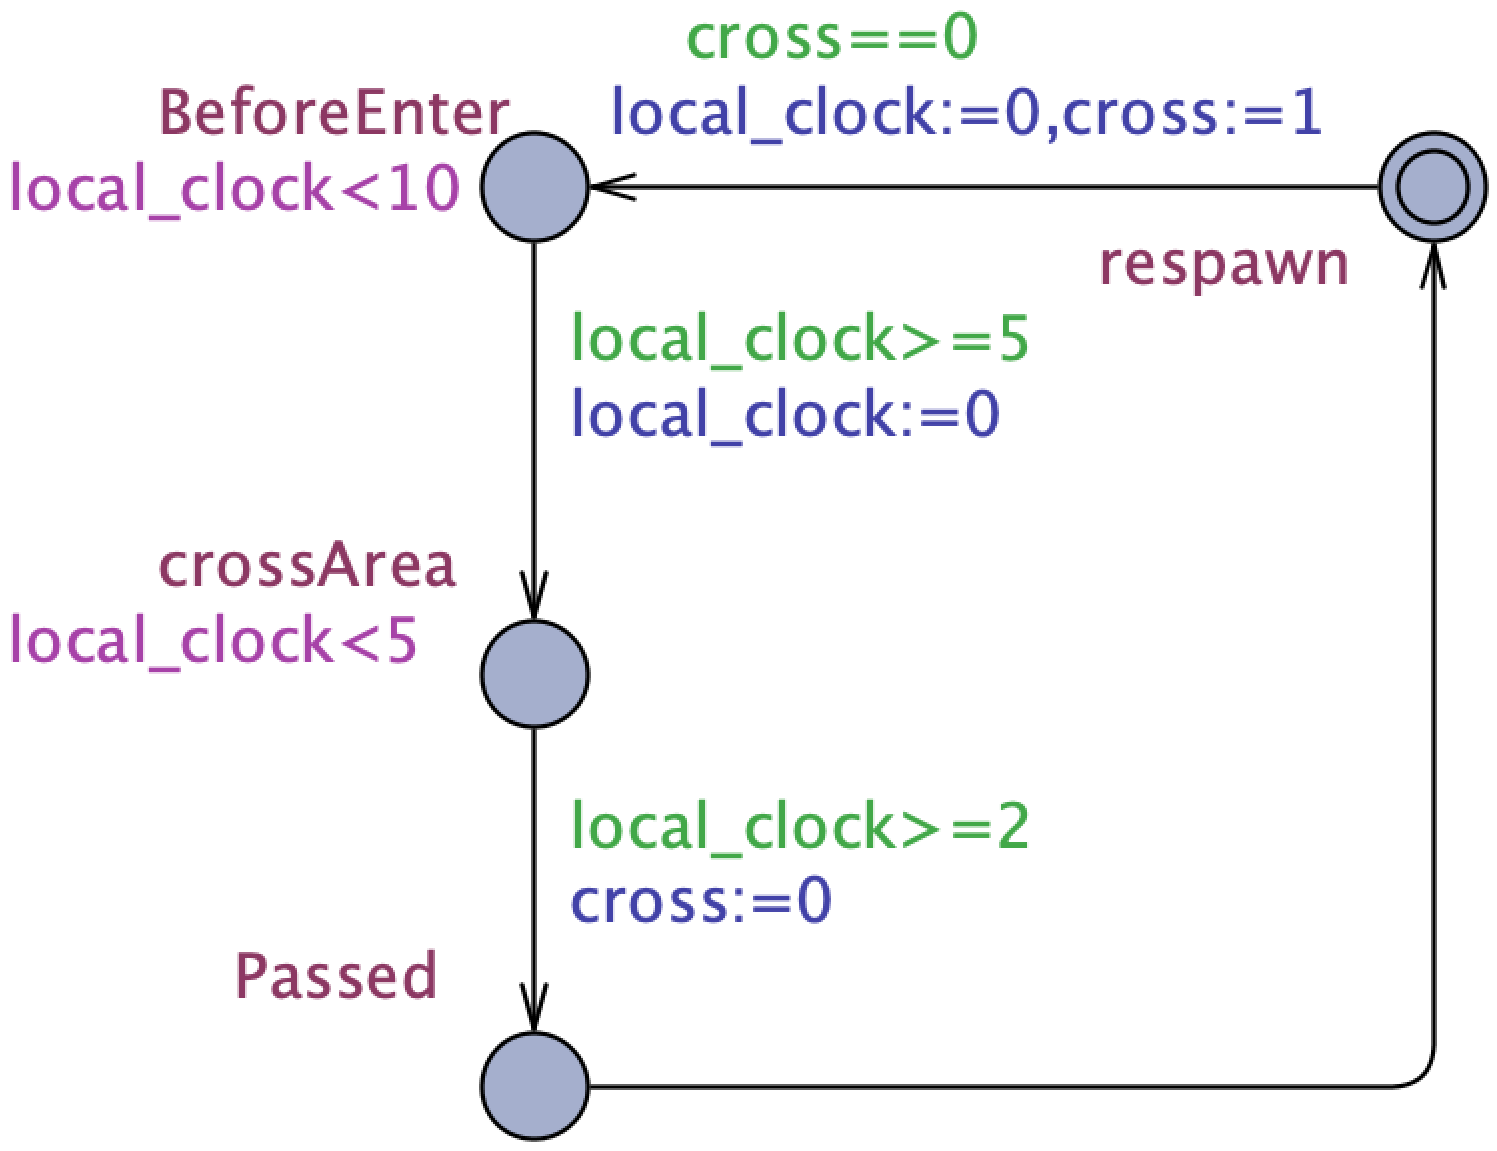
\includegraphics[width=125mm]{Perpendicular.png}
	\caption{交差点進入時に使用権を取得する車両1台の時間オートマトン}
	\label{Perpendicular}
	\end{figure}
	
	図\ref{PerpendicularS}は時間オートマトン表現で進行方向が垂直に交わる2台の車両の現在状態である。便宜的に左のプロセスverticalを南北方向に直進してるとし,右のプロセスhorizonを東西方向に直進しているとする。現在状態はverticalが交差点の使用権を獲得し,進入前状態で,horizonが交差点通過後の状態である。
	\begin{figure}[htbp]
	\centering
	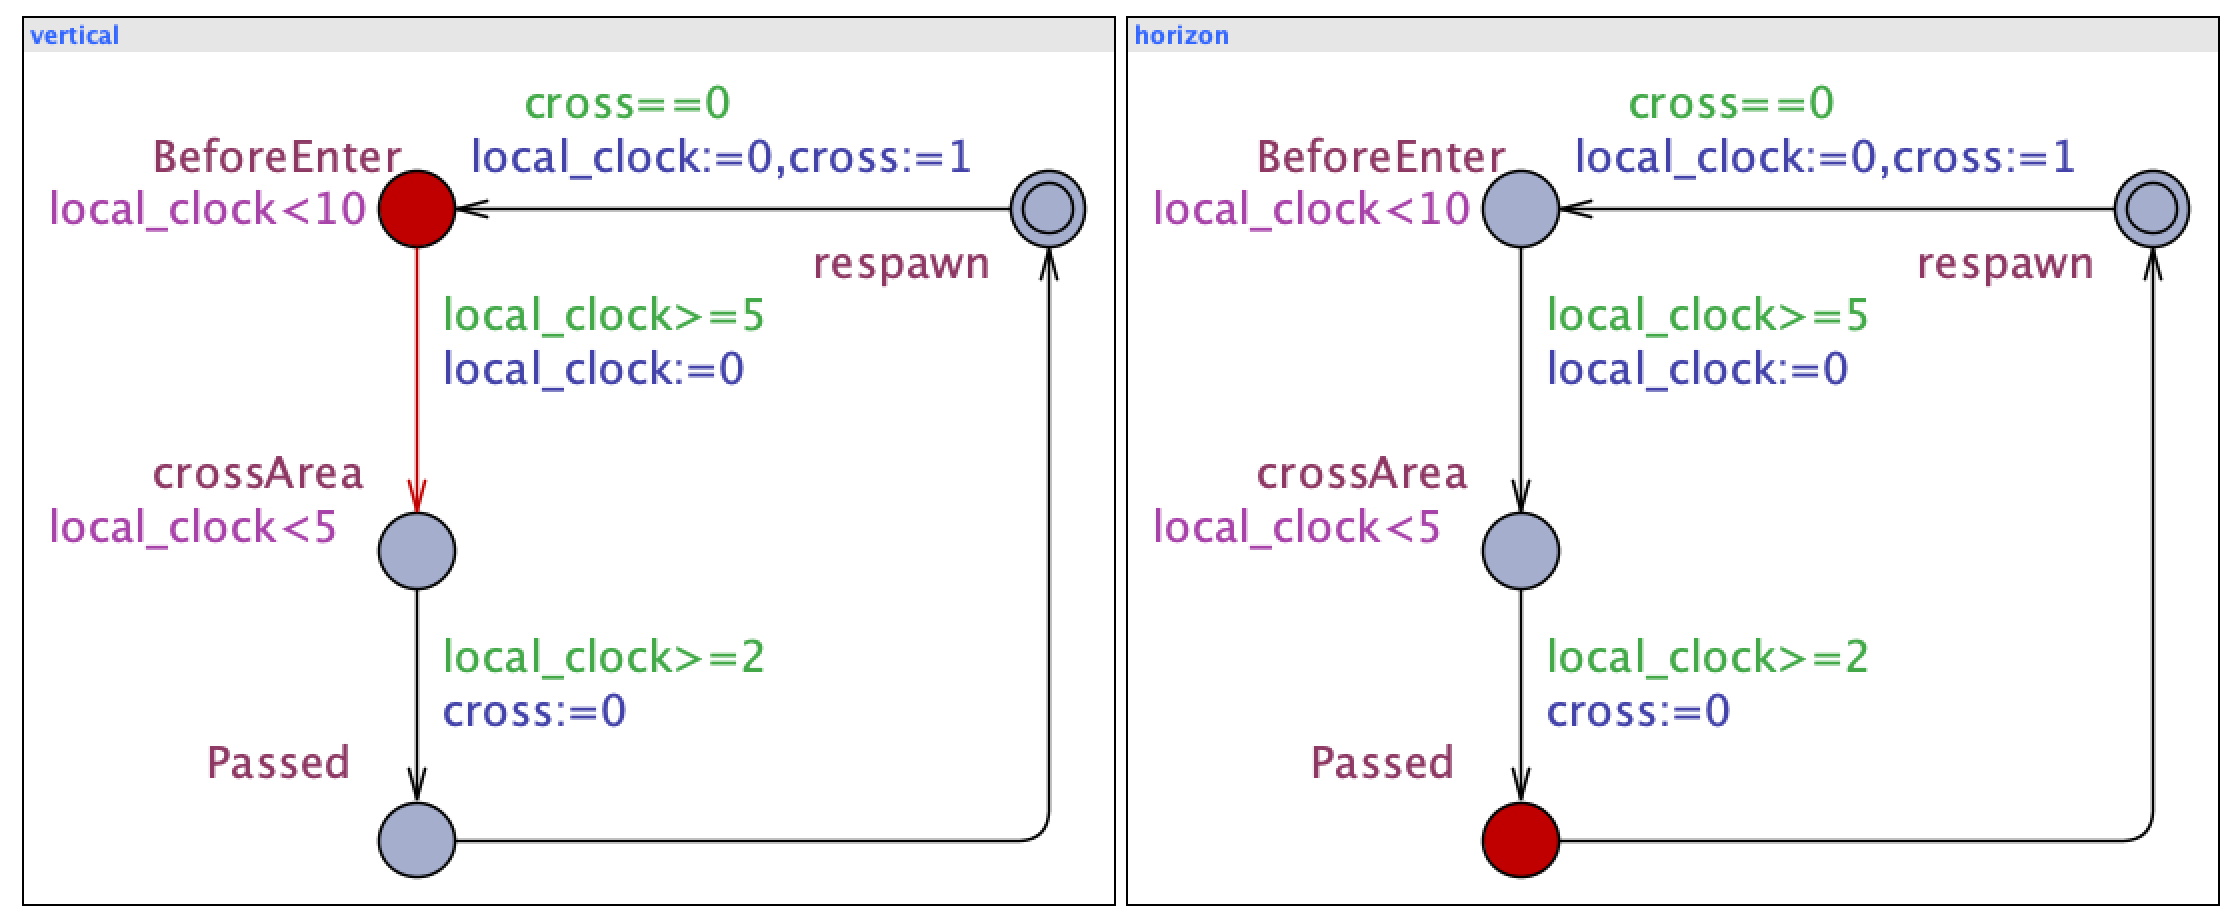
\includegraphics[width=130mm]{PerpendicularSimu.png}
	\caption{垂直に交差点に進入する車両の時間オートマトンの合成}
	\label{PerpendicularS}
	\end{figure}
	
	このモデルでデッドロック検証を行うと0.001秒未満の時間で検証できた。s

	
	\subsection{東西南北それぞれから交差点に直進する時間オートマトン}
	直進して交差点を通過する車両の進行方向に対して,他の車両の進行方向が垂直であったり,平行であったりする時の交差点の使用権の獲得方法を考える。前例では,crossが交差点の使用権そのものでそれの有無で進入を決定していたが,本例では,進行方向が平行となる場合は同時に進入可能としたい。したがって交差点の使用権を図\ref{oTWoL}に示すように4つの鍵の組み合わせで管理したい。例えば,西から東へ進行する車両はlock1とlock2を取得する。北から南へ進行する車両はlock2とlock4を取得しようとするが,既にlock2が取得されているためこの車両は交差点へ進入できない。一方で前者に対して,東から西へ進行する車両はlock3とlock4を取得できるため,交差点へ進入する。
	\begin{figure}[htbp]
	\centering
	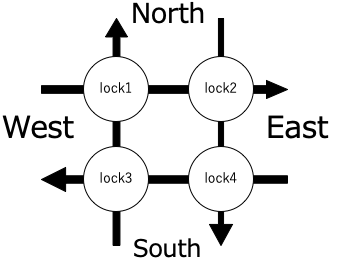
\includegraphics[width=100mm]{onTheWayofLock.png}
	\caption{交差点の使用権を管理する4つの鍵の組み合わせ}
	\label{oTWoL}
	\end{figure}
	
	使用権を4つの鍵で管理する交差点に直進する車両の時間オートマトンを作成する(図\ref{news})。遷移可能条件をパラメータ(L1,L2)で記述し,それぞれが取得する鍵に紐付けている。初期状態respawnから交差点進入前状態BeforeEnterへ遷移時にふたつの鍵L1とL2を1に更新して使用権を取得する。前例と同様にこのオートマトンも直進のみのため,タイマーであるlocal\_clockは同内容を記述している。交差点通過中状態crossAreaから交差点通過後状態Passedへの遷移時に鍵の解除としてL1==0とL2==0と記述した。
	
	北から南へ直進する車両をsn,南から北へ直進する車両をns,東から西へ直進する車両をew,西から東へ直進する車両をweとして,図\ref{newsS}では,ewが交差点を交差点通過中で,lock3とlock4が取得されている。lock1とlock3を取得できたweが交差点進入前状態である。
	\begin{figure}[htbp]
	\centering
	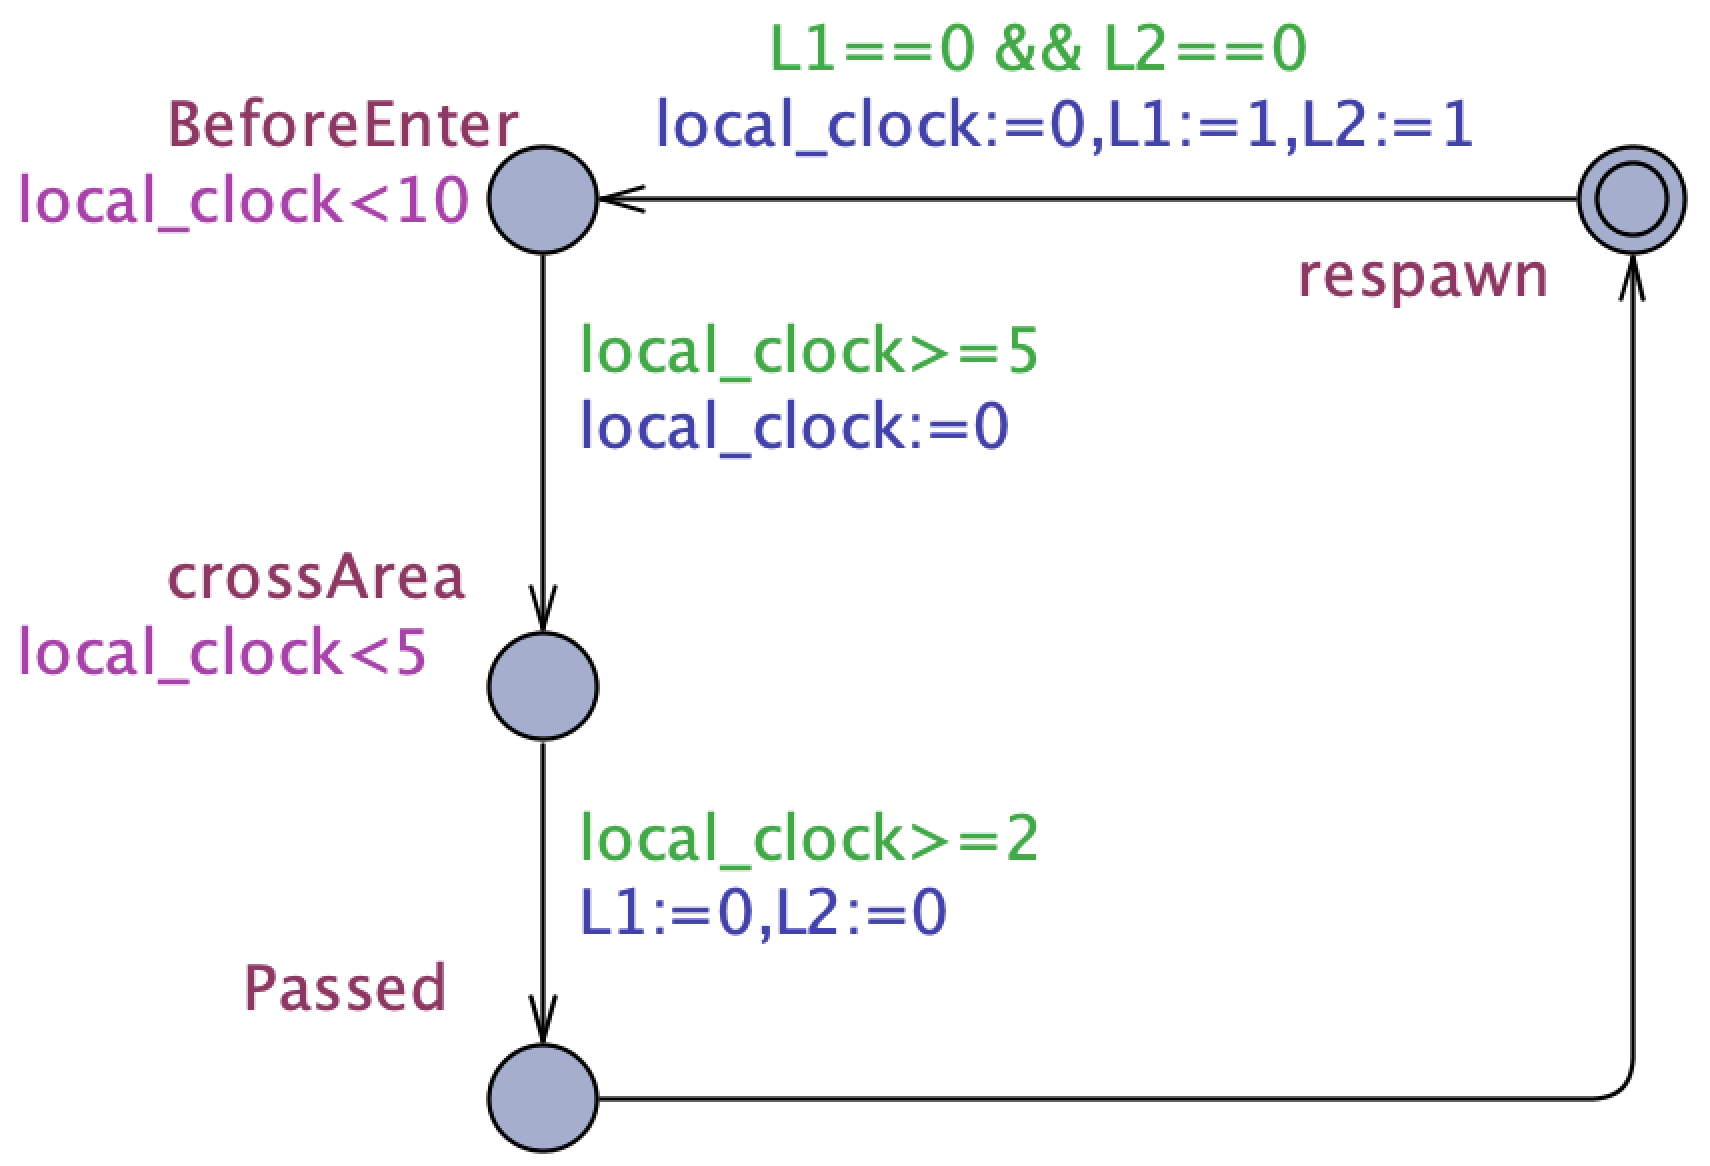
\includegraphics[width=130mm]{news.png}
	\caption{使用権を4つの鍵で管理する交差点に直進する車両の時間オートマトン}
	\label{news}
	\end{figure}
	\begin{figure}[htbp]
	\centering
	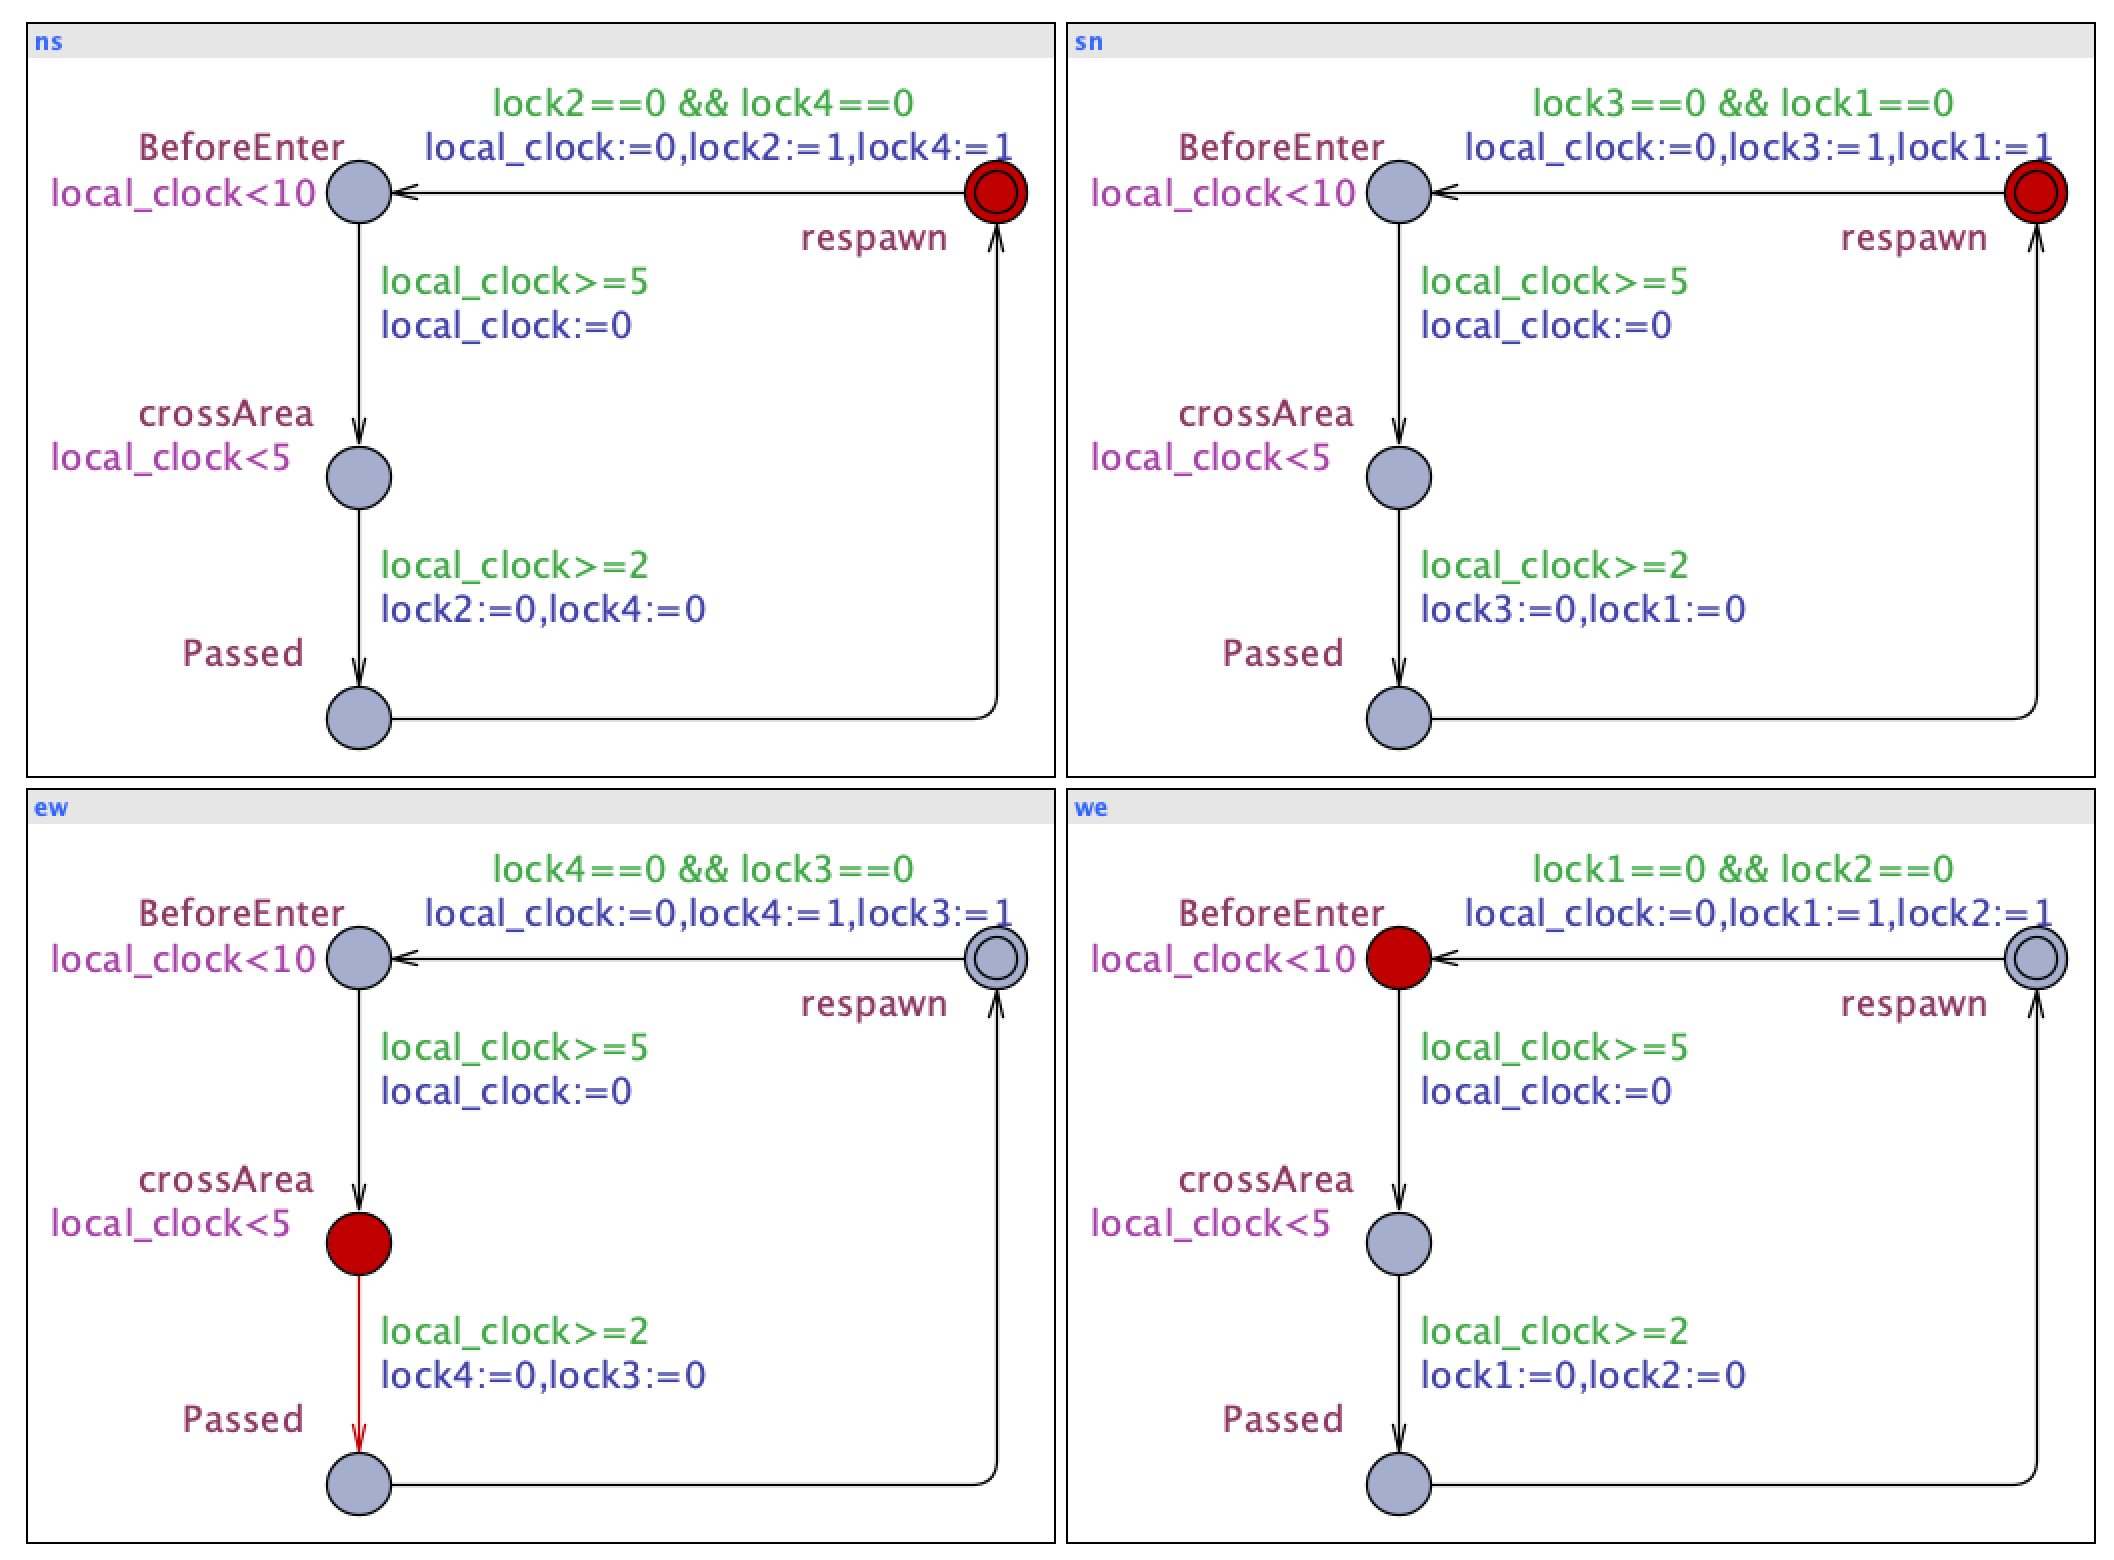
\includegraphics[width=130mm]{newsSimu.png}
	\caption{交差点に直進する車両の時間オートマトンの合成}
	\label{newsS}
	\end{figure}
	
	
	\subsection{交差点を直進・左折・右折する車両の時間オートマトン}
	交差点を直進する車両と左折する車両と右折する車両を考慮した時間オートマトンを作成する(図\ref{Simple})。前述までとは違い,右折する場合もあるため,4つの鍵の組み合わせでは右折する車両同士での衝突が起こる可能性がある。したがって前述の4つの鍵に加えて,右折用の鍵crossを用意する。鍵crossは3つ目のパラメータuseの値と照らし合わせる。パラメータuseは右折用の鍵を使用するかどうかを車両の固定情報として保持している。初期状態respawnから交差点進入前状態BeforeEnterへの遷移可能条件をパラメータL1,L2,右折用鍵crossが取得可能であることとした。また,左折時は,パラメータは2つあるが,取得する鍵は1つである。そのため,南から東へ右折する車両と,東から南へ左折する車両と,西から北へ左折する車両の3台が同時に交差点に進入可能となっている。本オートマトンでは,右折や左折が直進より時間がかかることとし,時間に関する条件は前述までのモデルより長くした。
	
	北から南へ直進する車両をsn,南から北へ直進する車両をns,東から西へ直進する車両をew,西から東へ直進する車両をwe,北から東へ左折する車両をne,南から西へ左折する車両をsw,東から南へ左折する車両をes,西から北へ左折する車両をwn,北から西へ右折する車両をsw,南から東へ右折する車両をse,東から北へ右折する車両をen,西から南へ右折する車両をwsとすると,上記の3台の車両が交差点に進入する例が図\ref{SimpleS}のように,右折するseが通過中状態crossAreaの時,左折するesも状態crossAreaで,もう一つのwnが状態BeforeEnterとなっている。
	\begin{figure}[htbp]
	\centering
	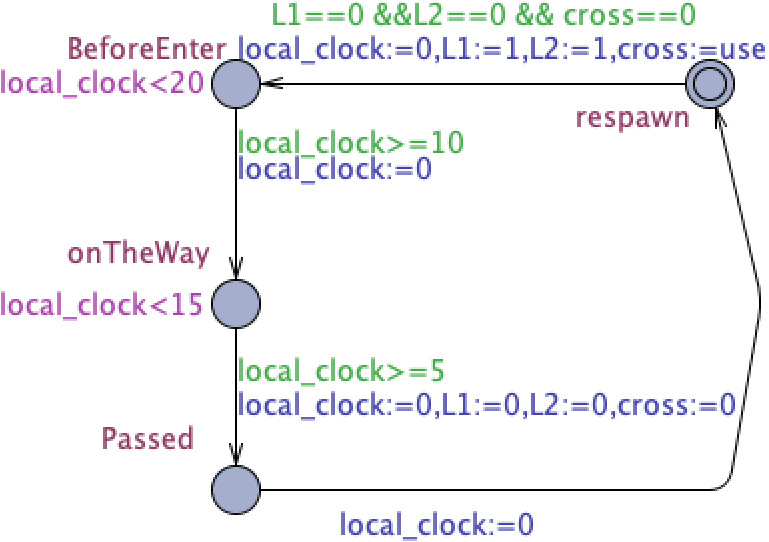
\includegraphics[width=140mm]{SimpleIntersection.png}
	\caption{交差点を通過する車両の時間オートマトン}
	\label{Simple}
	\end{figure}
	\begin{figure}[htbp]
	\centering
	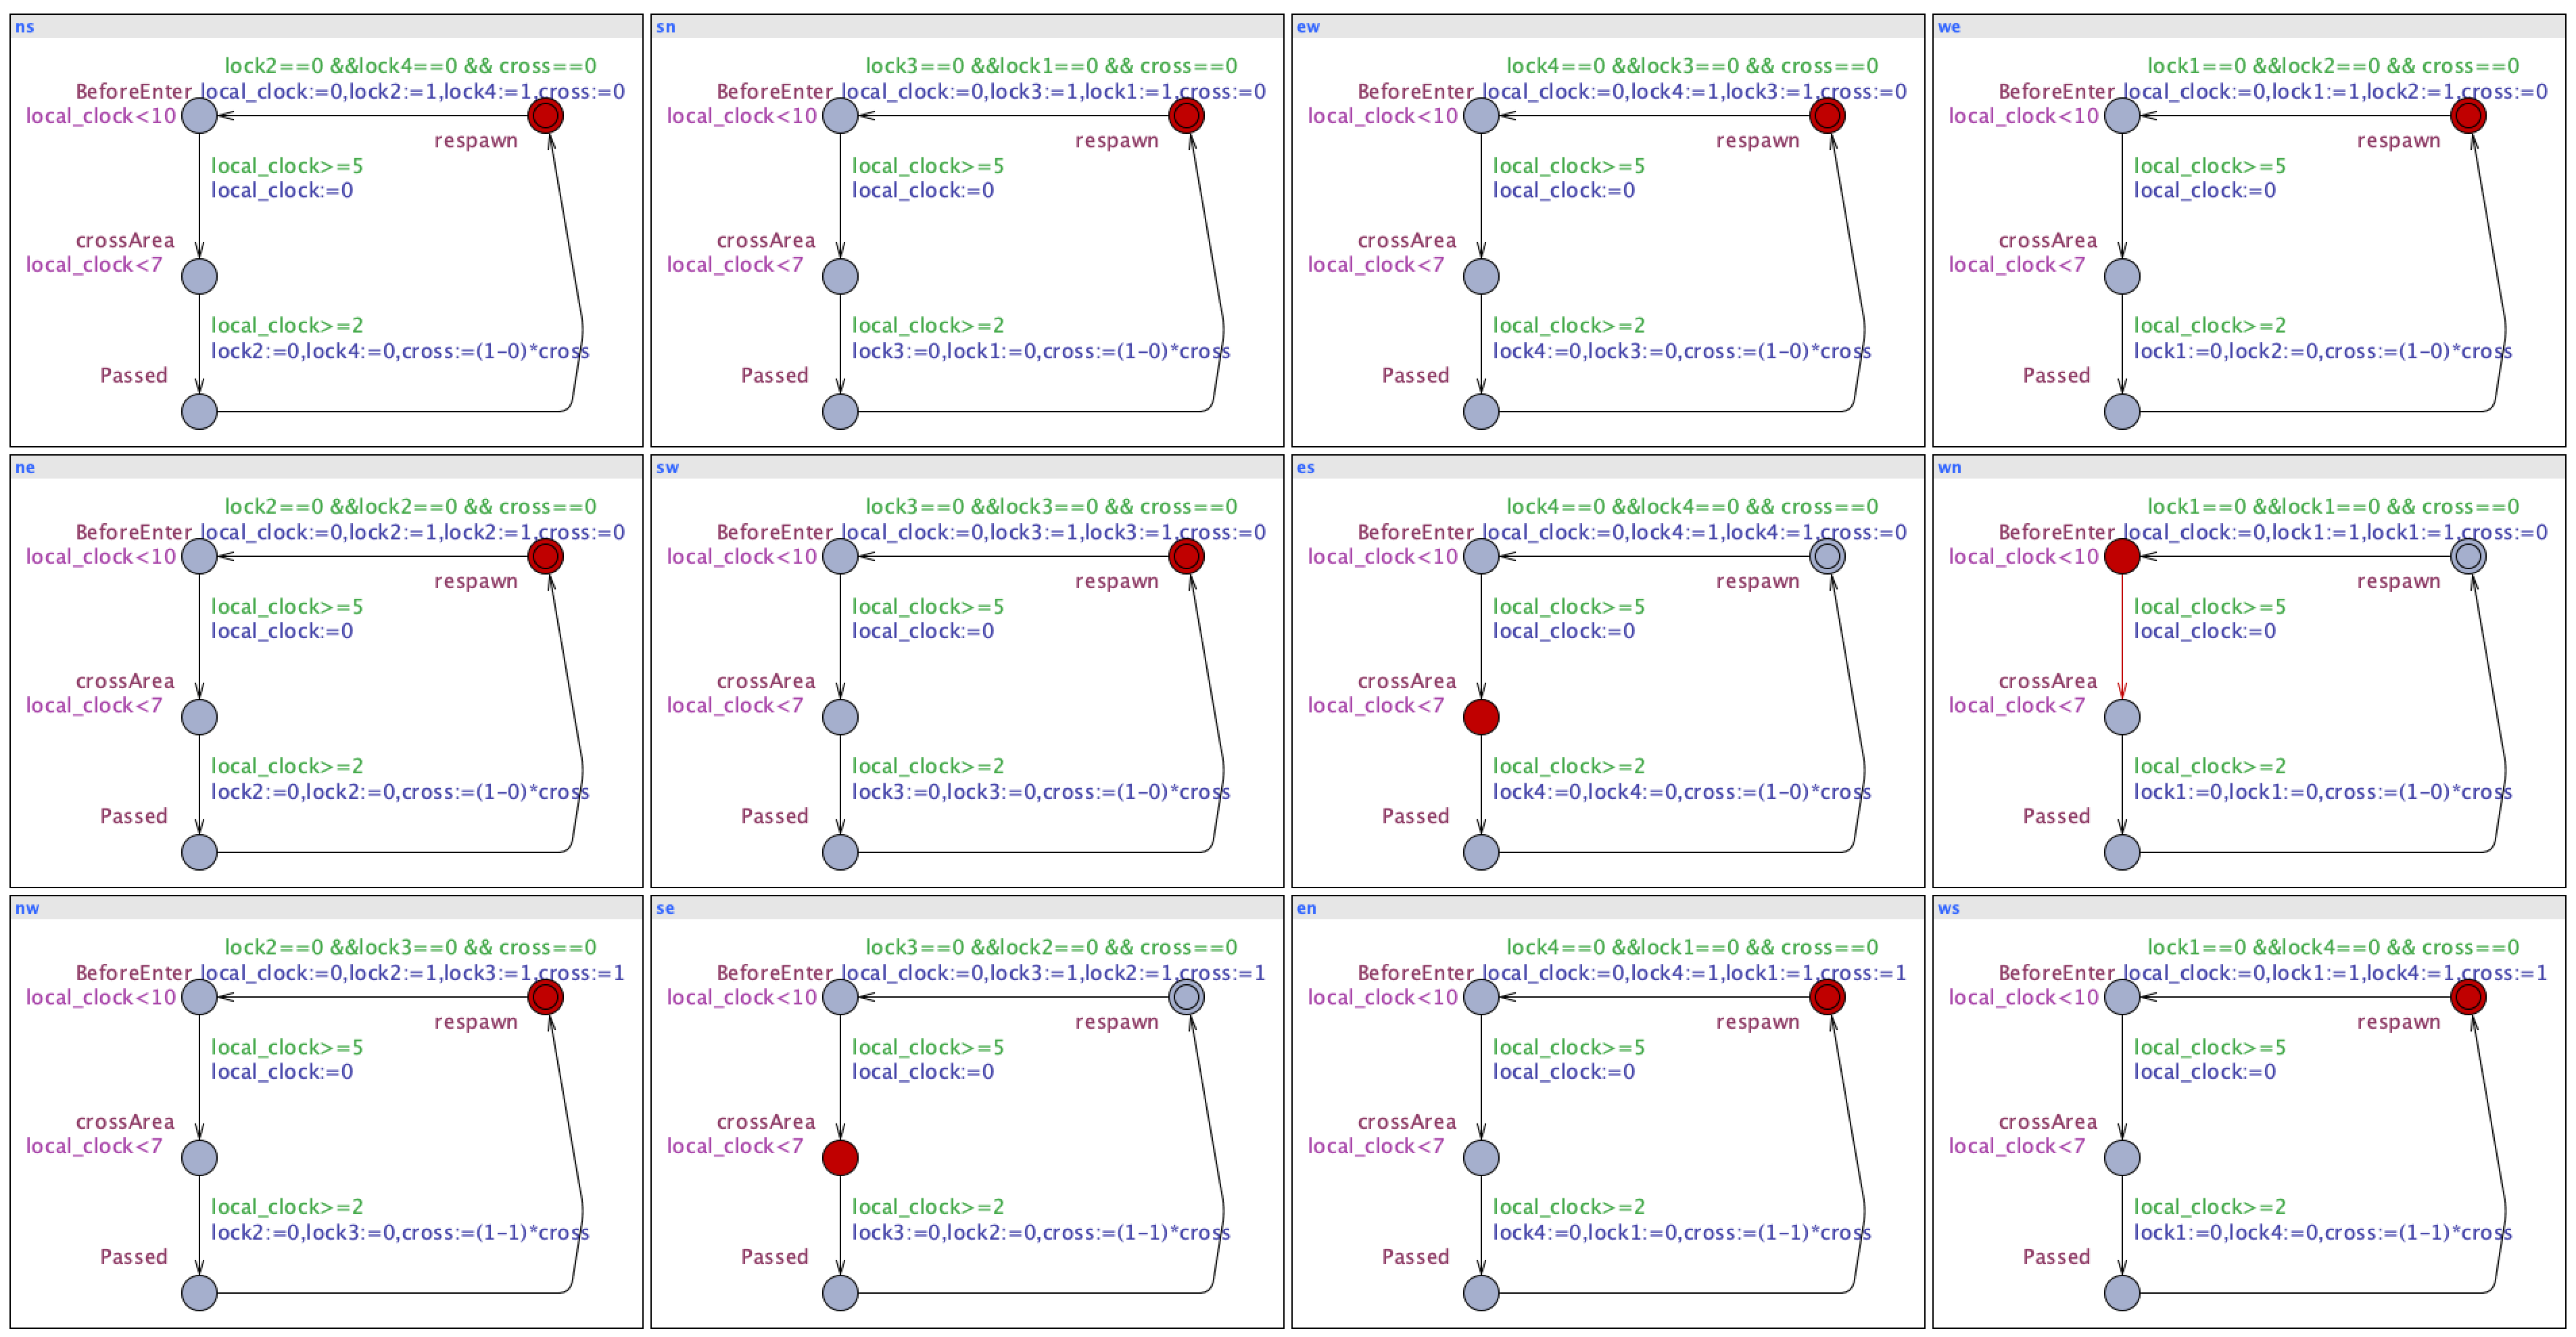
\includegraphics[width=150mm]{SimpleIntersectionSimu.png}
	\caption{交差点を通過する車両の時間オートマトンの合成}
	\label{SimpleS}
	\end{figure}
	
	
	\section{交差点の通過にかかる最小時間の検証}
	本節では,車両全てが交差点を1回通過するのにかかる最小時間について検証を行う。交差点の使用権の取得方法は前節と同仕様の5つ鍵によって管理する。1回だけなので循環するオートマトンではなく一方通行的なオートマトンを作成する(図\ref{minT})。初期状態startから交差点進入前状態BeforeEnterへの遷移可能条件に交差点の使用権の取得として,L1==0かつL2==0かつcross==0を与える。状態BeforeEnterから交差点通過中状態crossAreaへの遷移可能条件とBeforeEnterの状態不変条件で交差点進入前7秒以上10秒未満の間で使用権を獲得しなければならないかを記述し,状態crossAreaから交差点通過後である終了状態finishへの遷移可能条件とcrossAreaの状態不変条件で交差点の通過にかかる時間を記述し,crossAreaからfinishへの状態遷移時に使用権の解除を行う。
	
	検証したい性質の導出:
	
	検証式
	
	検証結果
	\begin{figure}[htbp]
	\centering
	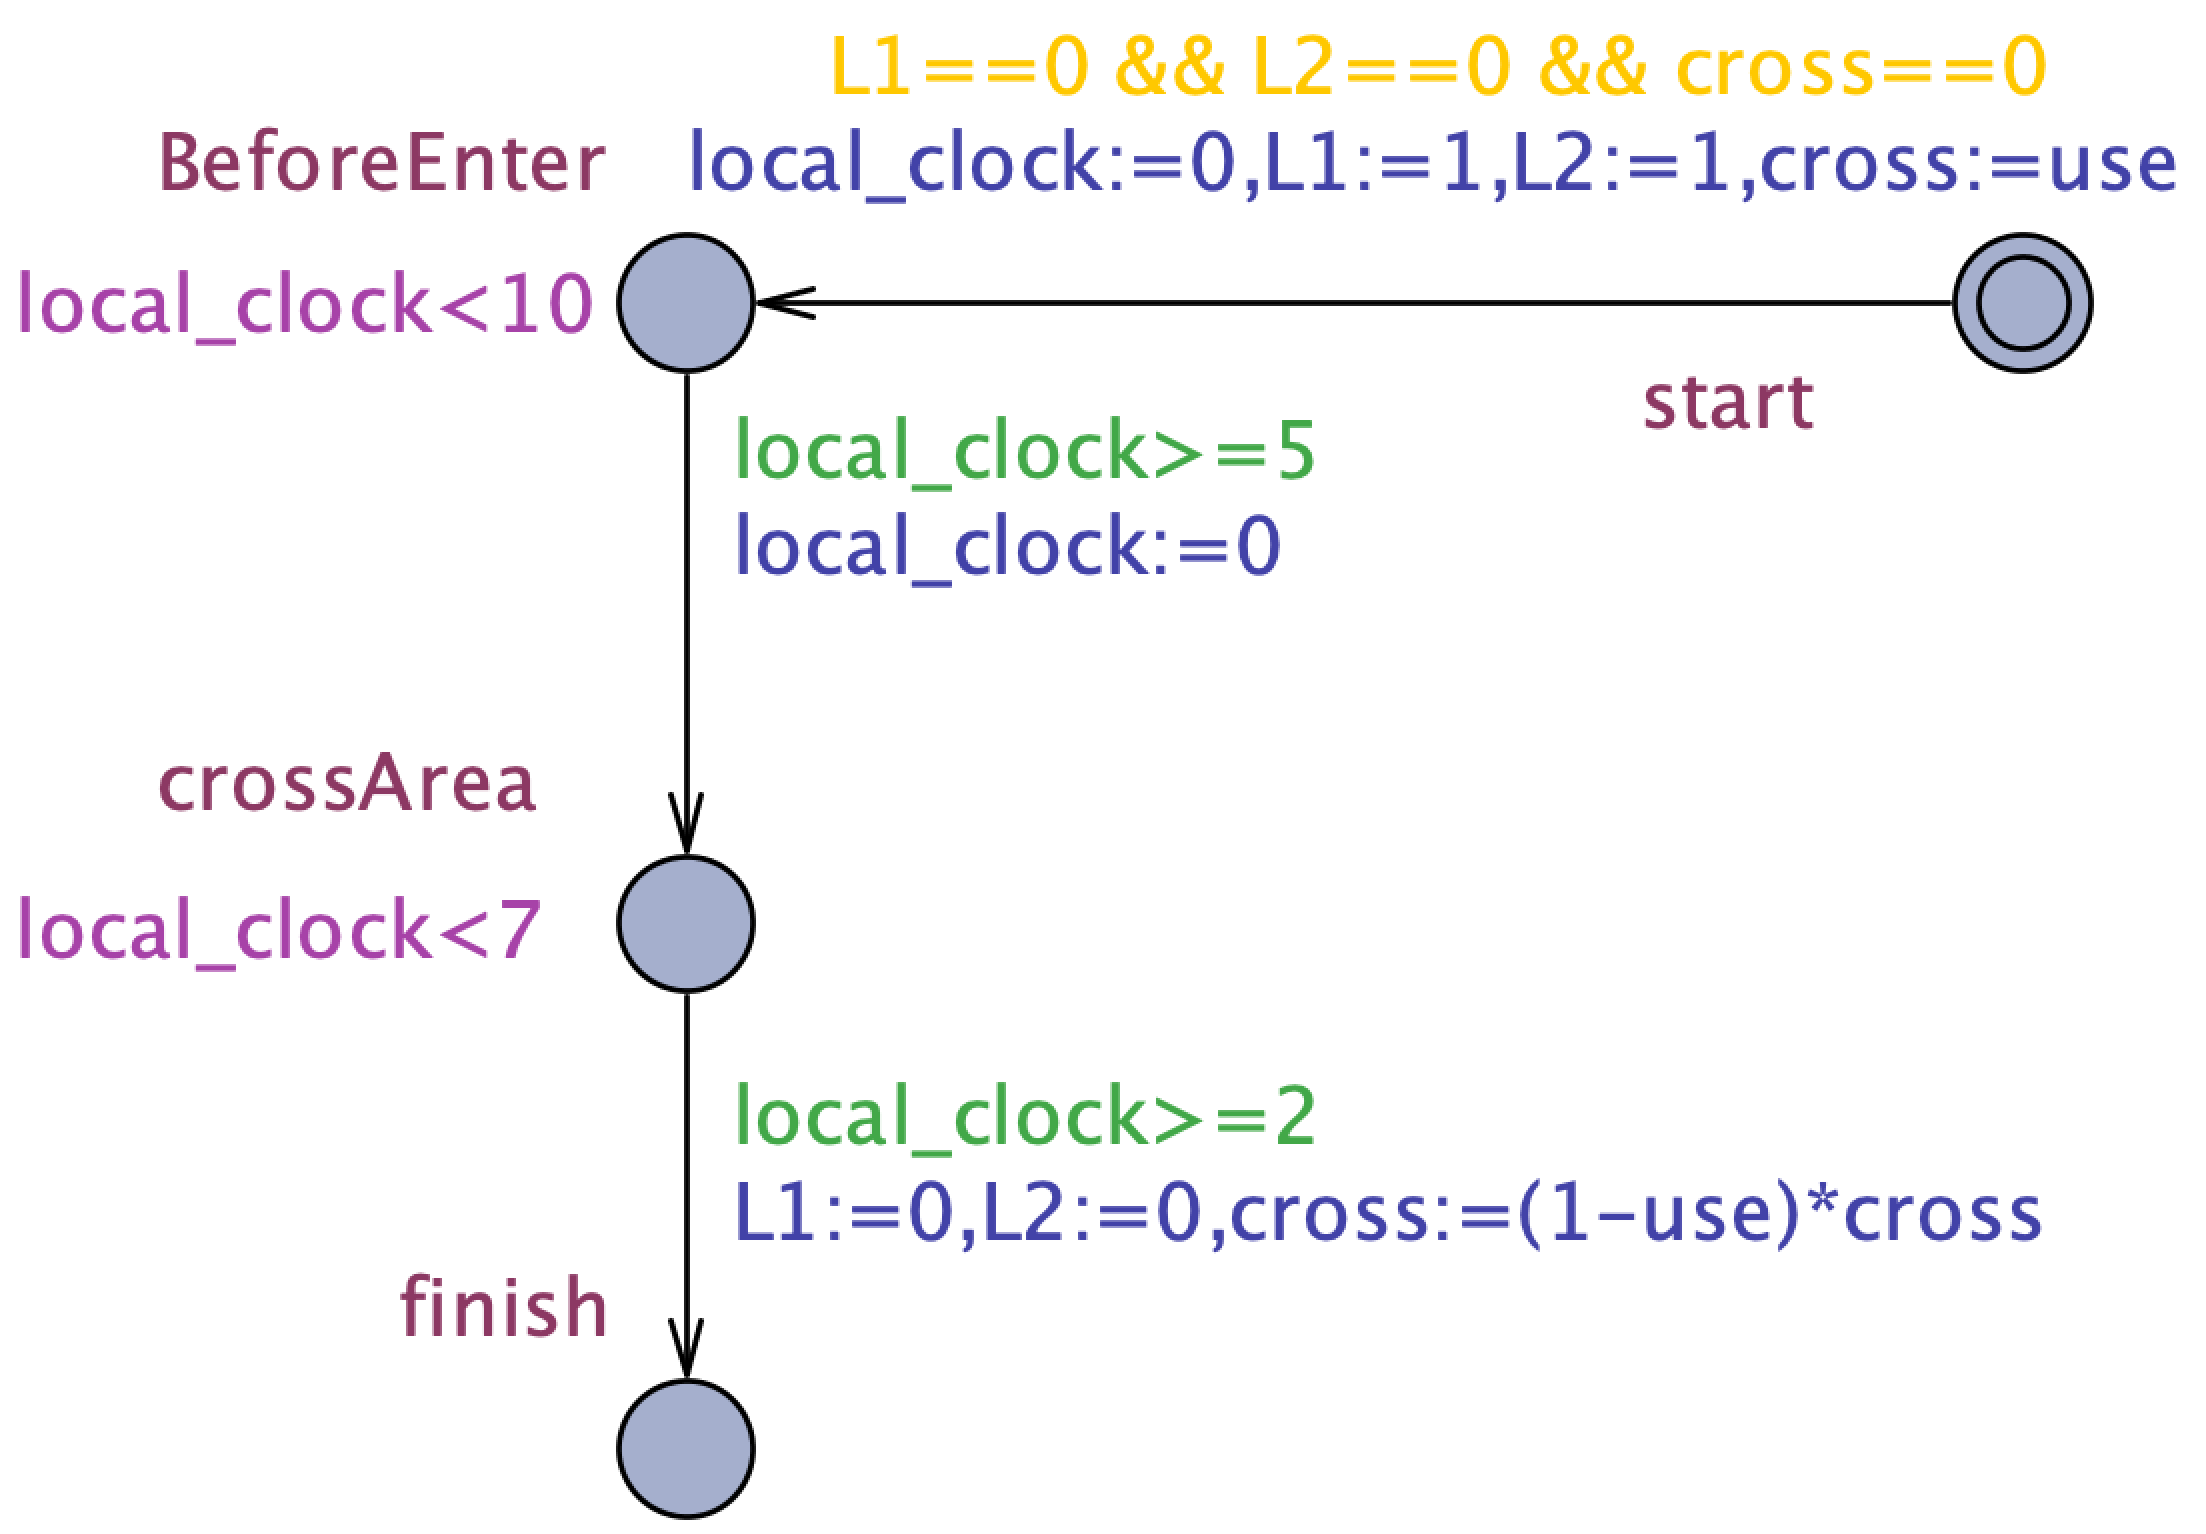
\includegraphics[width=130mm]{minTime.png}
	\caption{交差点を1回通過する時間オートマトン}
	\label{minT}
	\end{figure}
%\chapter{考察}

\chapter{おわりに}
本研究では,UPPAALを用いた自動運転車群制御アルゴリズムのモデル化と検証の手法を提案した。単一の交差点においては車両の挙動をモデル化し,デッドロックや通過時間を検証することができた。複数の交差点から構成される都市空間のモデルを作成し検証することが今後の課題である。
\acknowledgements
本研究を進める上で,多くのご助言とご指摘をいただきました中村准教授,榊原准教授に心より感謝の意を表します。また,多くの助言と協力をいただきました中村研究室,榊原研究室の皆様にも深く感謝いたします。
\begin{thebibliography}{9}
	\bibitem{a1}{長谷川哲夫,田原康之,磯部祥尚, UPPAALによる性能モデル検証ーリアルタイムシステムのモデル化と検証ー, 近代科学社, 2012.}
	\bibitem{Nu}{A. Cimatti, E. M. Clarke, E. Giunchiglia, F. Giunchiglia, M. Pistore, M. Roveri, R. Sebastiani and A. Tacchella,NuSMV 2: An OpenSource Tool for Symbolic Model Checking,In Proceeding of International Conference on Computer-Aided Verification (CAV 2002), pp. 359-364, 2002.}
	\bibitem{n2}{NuSMV home page, \verb$http://nusmv.fbk.eu$}
	\bibitem{s1}{G.J. Holzmann, The SPIN Model Checker: Primer and Reference Manual, Addison-Wesley, 2003.}
	\bibitem{s2}{Spin - Formal Verification, \verb$http://spinroot.com$}
	\bibitem{u1}{Uppaal in a Nutshell. Kim G. Larsen, Paul Pettersson and Wang Yi. In Springer International Journal of Software Tools for Technology Transfer 1(1+2), 1997.}
	\bibitem{u2}{UPPAAL, \verb$http://www.uppaal.org$}
	\bibitem{u3}{Timed Automata: Semantics, Algorithms and Tools, Johan Bengtsson and Wang Yi. In Lecture Notes on Concurrency and Petri Nets. W. Reisig and G. Rozenberg (eds.), LNCS 3098, Springer-Verlag, 2004.}
	\bibitem{a9}{綿引健二, 石川冬樹, 平石邦彦, 時間, 資源の制約をもつビジネスプロセスの形式検証, 電子情報通信学会論文誌 D, 96(8):1878-1891, 2013.}
\end{thebibliography}
\end{document}